\section{Quantum Mechanics}
\subsection{Symbols and Notation}
\begin{itemize}
    \item $p$ -- momentum (impulse), measured in $\mathrm{kg\,m/s}$
    \item $m$ -- mass of the particle, measured in $\mathrm{kg}$
    \item $v$ -- velocity of the particle, measured in $\mathrm{m/s}$
    \item $E$ -- energy, measured in $\mathrm{J}$
    \item $h$ -- Planck's constant, $6.626 \times 10^{-34}\,\mathrm{J\,s}$
    \item $f$ sometimes $v$ -- frequency, measured in $\mathrm{Hz}$
    \item $c$ -- speed of light in vacuum, $2.998 \times 10^8\,\mathrm{m/s}$
    \item $\lambda$ -- wavelength, measured in $\mathrm{m}$
    \item $\hbar$ -- reduced Planck's constant, $\hbar = \frac{h}{2\pi}$
    \item $\psi(x)$ -- wave function (probability amplitude)
    \item $|\psi(x)|^2$ -- probability density at position $x$
    \item \(eV\) -- electronvolt, a unit of energy, \(1\,eV = 1.602 \times 10^{-19}\,\mathrm{J}\)
\end{itemize}
\begin{equation*}
    p = m \cdot v
\end{equation*}
Photon:
\begin{equation*}
    E = h \cdot f = \frac{h \cdot c}{\lambda}
\end{equation*}
De Broglie wavelength:
\begin{equation*}
    \lambda = \frac{h}{p} = \frac{h}{m \cdot v}
\end{equation*}
\subsection{Schrödinger equation}
The time-independent Schrödinger equation:
\begin{equation*}
    \label{eq:time-independent-schroedinger}
\left(-\frac{\hbar^2}{2m} \frac{d^2}{dx^2} + V(x)\right) \psi(x) = E \psi(x),
\end{equation*}

\(\psi(x)\) is a probabilty amplitude which doesnt say much itself. Only \(|\psi(x)|^2\) which is a probabilty density.
\cref{eq:time-independent-schroedinger} can be transformed to 
\begin{equation*}
    \frac{d^2}{dx^2} \psi(x) - b^2 \cdot \psi(x) = 0
\end{equation*}
which can be solved by
\begin{equation*}
    \psi(x) = A_1 \cdot e^{b \cdot x} + A_2 \cdot e^{-b \cdot x}
\end{equation*}
\begin{equation*}
    b = \sqrt{\frac{2m}{\hbar^2}\cdot (V-E)}
\end{equation*}
If \(V > E\), then \(b\) is imaginary and the solution is
\begin{equation*}
    \psi(x) = A_1 \cdot \sin(k \cdot x - \varphi)
\end{equation*}
with
\begin{equation*}
    k =\frac{2\pi}{\lambda} =  \sqrt{\frac{2m}{\hbar^2}\cdot (E-V)}.
\end{equation*}
Else if \(V < E\), then \(b\) is real and the solution is
\begin{equation*}
    \psi(x) = A_2 \cdot e^{-b \cdot x}
\end{equation*}
which is a real exponential decay.

Heisenberg's uncertainty principle:
\begin{equation*}
    \Delta x \cdot \Delta p \geq \frac{\hbar}{2}\quad \text{or}\quad \Delta E \cdot \Delta t \geq \hbar
\end{equation*}

\subsection{Wave Packet}
Gaussian superposition of different wace functions concentrated around a certain point \(k_0 \Rightarrow\) Gaussian envelope on space.
Single wave moves at phase velocity:
\begin{equation*}
    v_{phase} = \frac{\lambda}{T} = f \cdot \lambda = \frac{E}{p} = \frac{\hbar k}{m}
\end{equation*}
Wave packet moves with group velocity:
\begin{equation*}
    v_{group} = \left.\frac{d\omega}{dk}\right|_{k = k_0} = \frac{\hbar\, k_0}{m}
\end{equation*}
Due to dispersion \(\omega(k) = \frac{\hbar}{2\cdot m}\cdot k^2\), the following for the widths \(\sigma_k\) and \(\sigma_x\):
\begin{equation*}
    \sigma_k \cdot \sigma_x \ge \frac{1}{2}
\end{equation*}

\subsection{Infinite potential well}
Particle must remain inside the well \(\psi(0) = \psi(L) = 0\). Solution of Schrödinger Eqations: Standing waves.
\begin{equation*}
    \psi_n (x)  = \sqrt{\frac{2}{L}}\cdot\sin(n\cdot\frac{\pi}{L}\cdot x); n \in \mathbb{N}
\end{equation*}
Only certain \(k = n\cdot\frac{\pi}{L}\) and thus \(\lambda\) allowed:
\begin{equation*}
    E_n = n^2 \cdot \frac{\hbar^2 \pi^2}{2 m L^2} 
        = n^2 \cdot \underbrace{\frac{h^2}{8 m L^2}}_{= E_1} 
        = n^2 \cdot E_1
\end{equation*}

\subsection{Finite potential well}
\begin{figure}[h]
    \centering
    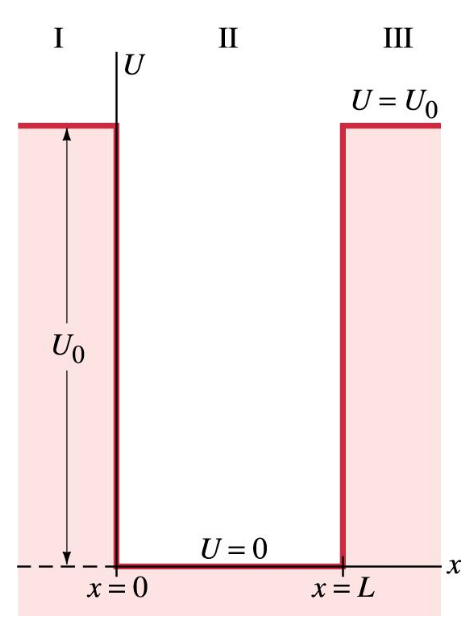
\includegraphics[width=0.4\columnwidth]{images/potentialwell.png}
    \label{fig:my_image}
\end{figure}
Potential energy to the left and right of the potential well is finite:
\begin{equation*}
 V = \,
\left\{
  \begin{array}{l}
    0 \qquad 0 \le x \le L \\
    U_{0}\qquad 0 < x\,\text{and} > L\\
  \end{array}
\right.
\end{equation*}
Three Areas \rom{1},\rom{2} and \rom{3}, in \rom{2} \((0 \le x \le L)\) particel is free:
\begin{equation*}
    \psi_{\rom{2}}(x) = A_{\rom{2}} \cdot \sin(k\cdot x - \varphi) \quad \text{with:}\quad k = \frac{2\pi}{\lambda} = \sqrt{\frac{2\cdot m}{\hbar^2}\cdot E}
\end{equation*}
but without the limitation \(\psi(0) = \psi(L) = 0\).
\textbf{For \(E \le U_0\) the following applies in areas \rom{1} and \rom{3}}:
\begin{equation*}
    \psi(x) = A_1 \cdot e^{b\cdot x} + A_2 \cdot e^{b\cdot x} \quad \text{with:}\quad b = \sqrt{\frac{2\cdot m}{\hbar^2}\cdot(U_0 - E)}
\end{equation*}
\begin{equation*}
    \psi_{\rom{1}} = A_{\rom{1}} \cdot e^{b\cdot x} \quad  \text{with} \quad A_{\rom{3}} \cdot e^{-b\cdot x} 
\end{equation*}
Exponential drop to the left and right. On the walls, both the wave function and its derivative must be continuous:
\begin{equation*}
    \left.\psi_{\rom{1},\rom{3}}\right|_{x = 0,L} =
    \left.\psi_{\rom{2}}\right|_{x = 0,L}
    \quad \text{and} \quad
    \left.\frac{d\psi_{\rom{1},\rom{3}}}{dx}\right|_{x = 0,L} =
    \left.\frac{d\psi_{\rom{2}}}{dx}\right|_{x = 0,L}
\end{equation*}

\textbf{If \(E > U_0\) the solution in the areas \rom{1} and \rom{3} is also a harmonic wave:}
\begin{equation*}
    \psi(x) = A\cdot \sin(k\cdot x-\varphi)\quad\text{with:}\quad k= \frac{2\pi}{\lambda} = \sqrt{\frac{2\cdot m}{\hbar^2}\cdot(E-U_0)}
\end{equation*}
The wavelength in these areas is greater than in area \rom{2}.
\subsubsection{Potential step \(E > U_0\)}
A part of the incident wave is reflected or transmitted at each transition. We know:
\begin{equation*}
    A_r = \frac{k_1 - k_2}{k_1 + k_2}\cdot A_{ein}, \quad A_t = \frac{2\cdot k_1}{k_1 + k_2} \cdot A_{ein}
\end{equation*}
So there is a certain probability that a particel will be reflected
\begin{equation*}
    R = \frac{(k_1 -k_2)^2}{(k_1 + k_2)^2}
\end{equation*}
We find the wave numbers
\begin{equation*}
    k = \frac{2\pi}{\lambda} = \sqrt{\frac{2 \cdot m}{\hbar^2}\cdot (E-U_0)}
\end{equation*}
\subsection{Quantum Tunnelling}
\begin{figure}[h]
    \centering
    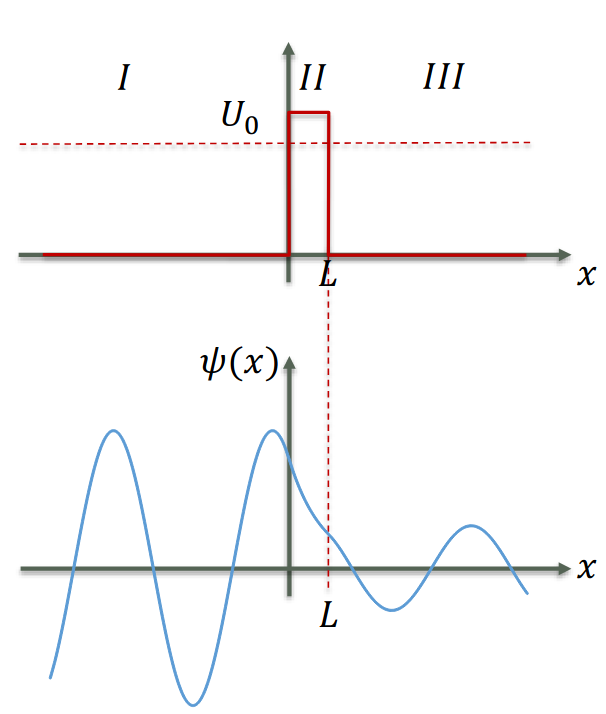
\includegraphics[width=0.4\columnwidth]{images/tunnel.png}
    \label{fig:tunnel}
\end{figure}
Exponential decrease with barrier with.
\begin{equation*}
    T \approx e^{-2\cdot b\cdot L} \quad\text{with:}\quad b = \sqrt{\frac{2\cdot m}{\hbar^2}\cdot (U_0 - E)}
\end{equation*}
Examples: Radiactive \(\alpha\) deacy, electron microscope
\subsection{Quantum harmonic oscillator}
\begin{figure}[h]
    \centering
    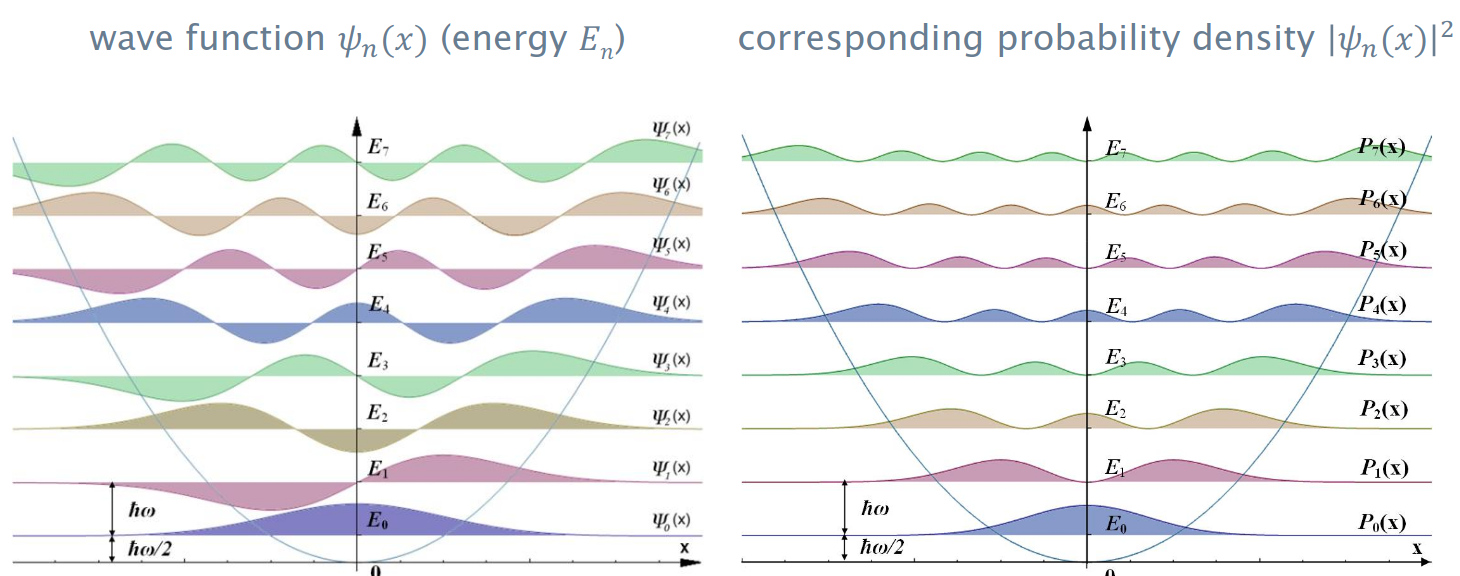
\includegraphics[width=\columnwidth]{images/harmoicoszillator.png}
    \label{fig:harmoszi}
\end{figure}
Complex math to get to \(\psi\).
Energy:
\begin{equation*}
    E_n = \hbar \cdot \omega\cdot (n + \frac{1}{2})\quad \text{with:}\quad n \in \mathbb{N}_0
\end{equation*}
Quantized, Equally spaced, Zero-point energy \(E_0 = \frac{1}{2}\hbar\omega\)
\begin{equation*}
    V(x) = \frac{1}{2}\cdot k \cdot x^2 = \frac{1}{2}\cdot m\cdot \omega^2 \cdot x^2
\end{equation*}
\section{Atoms}
For hydrogen atom, the potential (potential energy) is given by the spherically symmetric Coulomb potential:
\begin{equation*}
    V(r) = - \frac{1}{4\cdot \pi \cdot \epsilon_0}\cdot\frac{e^2}{r}
\end{equation*}
\(\epsilon_0\) permittivity of vacuum, \(e\) elemntary charge.

\begin{equation*}
    E_n = -\frac{m\cdot e^4}{8 \cdot \epsilon_0^2 \cdot h^2}\cdot\frac{1}{n^2}
    = -\frac{E_1}{n^2} = -\frac{13.6 \,\text{eV}}{n^2} 
\end{equation*}
with \(n = 1,2,3,\dots\).
Here \(n\) is the principal quantum number and defines the energy \(E_n\) belonging to the wave function \(\psi_{n.l,m}(r,\theta,\varphi)\)
\subsection{Quantum numbers}
\begin{itemize}
    \item \(n\) -- Principal quantum number (shell)
    \item \(l\) -- Azimuthal quantum number
    \item \(m_l\) -- Magentic quantum number
    \item \(m_s\) -- Spin quantum number (\(\pm \frac{1}{2}\)for electrons)
\end{itemize}

\subsection{Pauli exclusion principle}
Electrons as fermions (half integer spin)\(\rightarrow\) two electrons (inan atom) cannot be in the same quantum state.

\subsection{Molecules}
Two hydrogen atoms approach each other:
\begin{itemize}
    \item Parallel spins: \(S = \frac{1}{2} + \frac{1}{2} = 1\), Pauli principle \(\rightarrow\) No bond
    \item Antiparallel spins: \(S = \frac{1}{2} - \frac{1}{2} = 0\), Electron more likely inbetween nuclei \(\rightarrow\) attraction of the positiv nuclei to the electron cloud \(\rightarrow\) Covalent bond.
\end{itemize}
\subsection{Molecular (Organic) Semiconductors}
\begin{figure}[h]
    \centering
    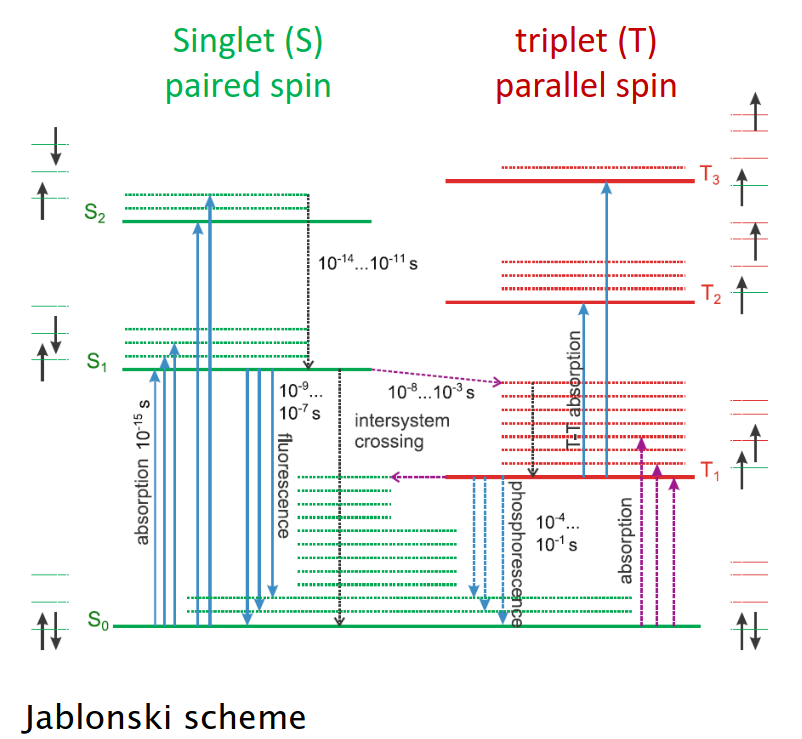
\includegraphics[width=\columnwidth]{images/jablonski.png}
    \label{fig:jablonski}
\end{figure}
\begin{itemize}
    \item Blue arrows: spin allowed transitions \(\rightarrow\) likely
    \item Dashed green and red lines: vibrational states
    \item Emission of photons mainly due to:
    \subitem Fluorescence (fast)
    \subitem Phosphorescence (slow)
\end{itemize}

\subsection{Electron Theory of Metals}
Electron are trapped in the metal like a potential well.
Within the metal(potential well) the potential energy is zero.
There are high potential walls at the metal edges.
Only a few electrons escape from the metal at room temperature(infinite potential well).
At higher temperatures electrons escape (thermal emmissions)(finite potential well).
In the potential well with macroscopic size, electrons can move freely.
Energy is quantized, distance between energy levels is very small (\(L\) very large).
\begin{equation*}
    E_n = n^2 \cdot \frac{h^2}{8 \cdot m \cdot L^2} = n^2 \cdot \frac{\hbar^2 \pi^2}{2\cdot m \cdot L^2} = n^2 \cdot E_1
\end{equation*}
Large number of states so close together that they seem to from a continuum.
Calculation of physical properties of conduction electrons by statistical meth ods.
Density of state \(g(E)\):
\begin{equation*}
    g(E) = \frac{8\sqrt{2}\pi m^{\frac{3}{2}}}{h^3}\sqrt{E}
\end{equation*}
\(g(E)\,dE\) indicates the number of states per volume unit that have energies between \(E\) and \(E + dE\).
\begin{figure}[h]
    \centering
    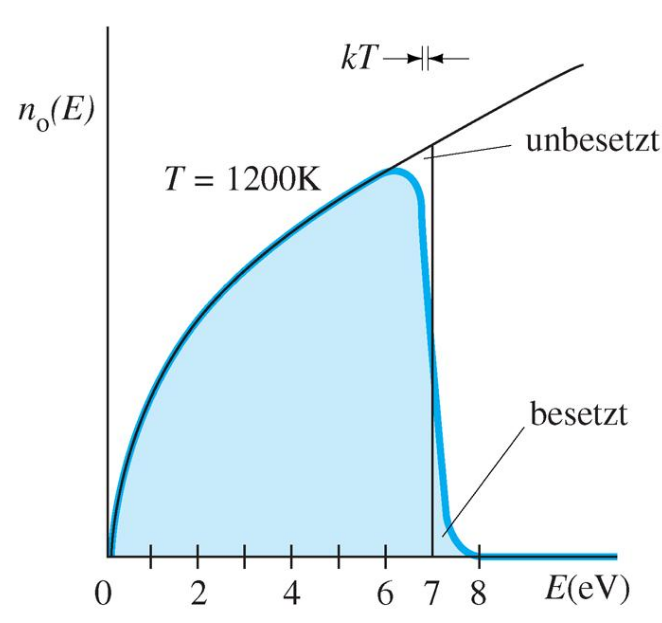
\includegraphics[width=0.8\columnwidth]{images/metals.png}
    \caption{Vertical black line: Fermi-Level}
    \label{fig:metals}
\end{figure}
Energy at Fermi level is called Fermi energy.
To determine the Fermi energy, we integrate from \(E = 0\) to \(E = E_F\):
\[
\frac{N}{V} = \int_{0}^{E_F}g(E)\, dE
\]
solving for \(E_F\):
\[
E_f = \frac{h^2}{8m}\left(\frac{3}{\pi}\frac{N}{V}\right)^{\frac{2}{3}}
\]
Mean energy:
\[
\overline{E} = \frac{3}{5}E_F
\]

In case of electron gas, a quantum mechanical system that is subject to the pauli principle, the occupation of a given state with that of the energy \(E\) is given by the Fermi-Dirac distribution:
\[
f(E) = \frac{1}{e^{(E-E_F)/kT} + 1}
\]
Occupation density:
\[
n_0(E) = g(E)\cdot f(E)
\]
\subsubsection{Calulations}
To approx \(N\)(Number of states) over a given range \(E + \Delta E\) and Volume \(V\). For exact values integrate \(g(E)\). For approximation take value in the middel(\(g(E + \frac{1}{2}\Delta E)\))
\begin{equation*}
    N \approx g(E + \frac{1}{2}\Delta E) \cdot V \cdot \Delta E
\end{equation*}
\subsection{Energy bands}
\begin{figure}[h]
    \centering
    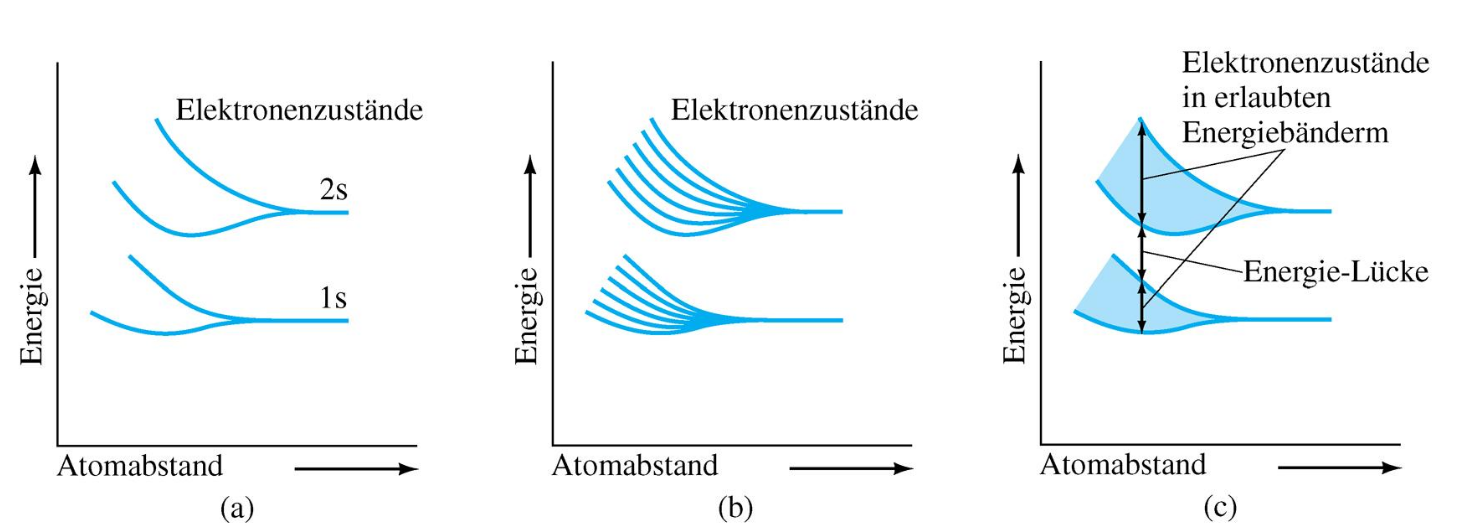
\includegraphics[width=\columnwidth]{images/bandmodel.png}
    \label{fig:bandmodel}
\end{figure}
The electrical conductivity of a crystal depends on how the highest energyband filled with electrons is filled: empty, partially filled, completely filled.
\begin{itemize}
    \item \textbf{Conductor:} The highest energy band occupied by electrons is only partially filled.
    \item \textbf{Insulator:} The highest band filled with electrons, the valence band, is completly filled.
    \item \textbf{Semiconductor:}The bands of a pure semiconductor are similar to those of an insulator, but the unfilled conduction band is seperated from the valence band by a much smaller band gap \(E_g\approx 1 \text{eV}\)
\end{itemize}
\subsubsection{Semiconductors}
Due to the small band gap, at room temperature, some electrons can absorb enough thermal energy to reach the conduction band, so that a very small current flows when voltage is applied.
The higher the temperature the more electrons overcome the band gap.
\begin{figure}[h]
    \centering
    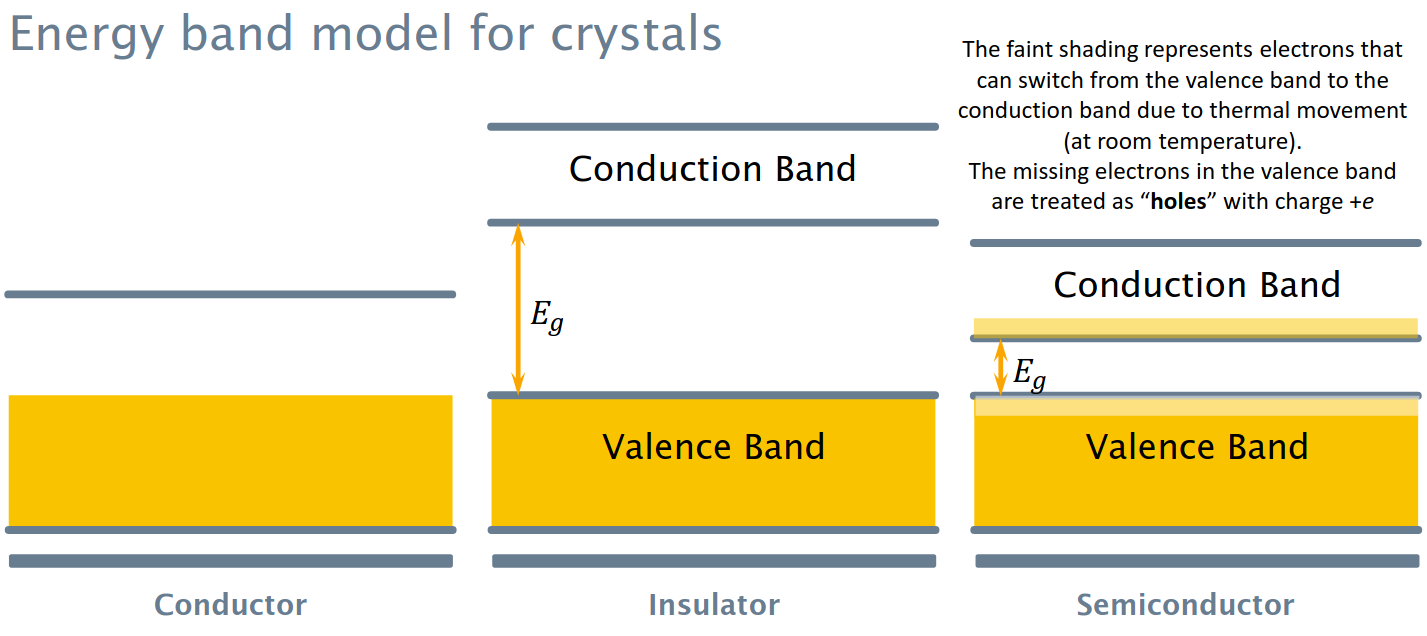
\includegraphics[width=\columnwidth]{images/bandmodel2.png}
    \label{fig:bandmodel2}
\end{figure}
\section{Absorption and emission}
\textbf{Black Body:}
\begin{itemize}
    \item Absorption = \(100\%\) for all wavelengths
    \item Emission:
    \subitem Thermal radiation
    \subitem Temperature dependent
    \subitem Planck's law 
\end{itemize}